\documentclass[11pt]{beamer}
\usetheme{Madrid}
\usecolortheme{default}
\setbeamertemplate{navigation symbols}{}
\setbeamertemplate{footline}[frame number]

\usepackage[utf8]{inputenc}
\usepackage{tikz}
\usetikzlibrary{shapes.geometric, arrows.meta, positioning, fit, backgrounds, decorations.pathreplacing}
\usepackage{booktabs}
\usepackage{array}

\title[Improving DTMIR-Pro]{All-Weather Image Restoration}
\subtitle{Improving DTMIR-Pro --- Progress Update 2}
\author{Pustak Pathak}
\institute{Advisor: Dr. Snehasis Mukherjee}
\date{Project Update}

\definecolor{kept}{RGB}{210,225,245}
\definecolor{changed}{RGB}{255,224,178}
\definecolor{newnode}{RGB}{198,239,206}
\definecolor{sidebox}{RGB}{238,238,238}
\definecolor{future}{RGB}{235,235,235}

\tikzstyle{block} = [rectangle, rounded corners, minimum width=6.6cm, minimum height=1.05cm,
  text centered, draw=black, align=center, font=\small]
\tikzstyle{futureblock} = [rectangle, rounded corners, minimum width=5.4cm, minimum height=1.0cm,
  text centered, draw=black, dashed, align=center, font=\scriptsize, fill=future]
\tikzstyle{arrowline} = [thick, -{Stealth[length=3mm]}]
\tikzstyle{dashedline} = [thick, dashed, -{Stealth[length=3mm]}, red!70!black]
\tikzstyle{futureline} = [thick, dashed, -{Stealth[length=2.5mm]}, gray]

\begin{document}

\begin{frame}
\titlepage
\end{frame}

\begin{frame}{What This Update Covers}
\begin{enumerate}
  \item A quick recap of the plan and the three changes
  \item What we actually \textbf{fixed in code} since last time
  \item Our first \textbf{visual result}: a training curve from a smoke run
  \item The \textbf{ablation ladder} we can now run for comparable numbers
  \item What we still need from the advisor / resources (GPU + data)
\end{enumerate}
\end{frame}

\begin{frame}{Quick Recap: What's Wrong With DTMIR-Pro Today}
DTMIR-Pro (our baseline) works in two steps: it first \textbf{translates} a degraded
image into a haze-look, a rain-look, and a snow-look version, then \textbf{restores}
the clean image using whichever of those three looks the closest to a known weather type.

\vspace{4mm}
Three weak points we identified:
\begin{itemize}
  \item[1] The translation step is trained once and then \textbf{frozen} --- it never
  learns from how well the final restoration actually turns out.
  \item[2] It can only describe an image as \textbf{100\% haze, 100\% rain, or
  100\% snow} --- real photos are often a mix of these.
  \item[3] It \textbf{throws away two out of three} translated versions and keeps
  only one, based on a rigid similarity rule.
\end{itemize}
\end{frame}

\begin{frame}{The Big Picture: Our Improved Pipeline}
\centering
\resizebox{!}{0.82\textheight}{
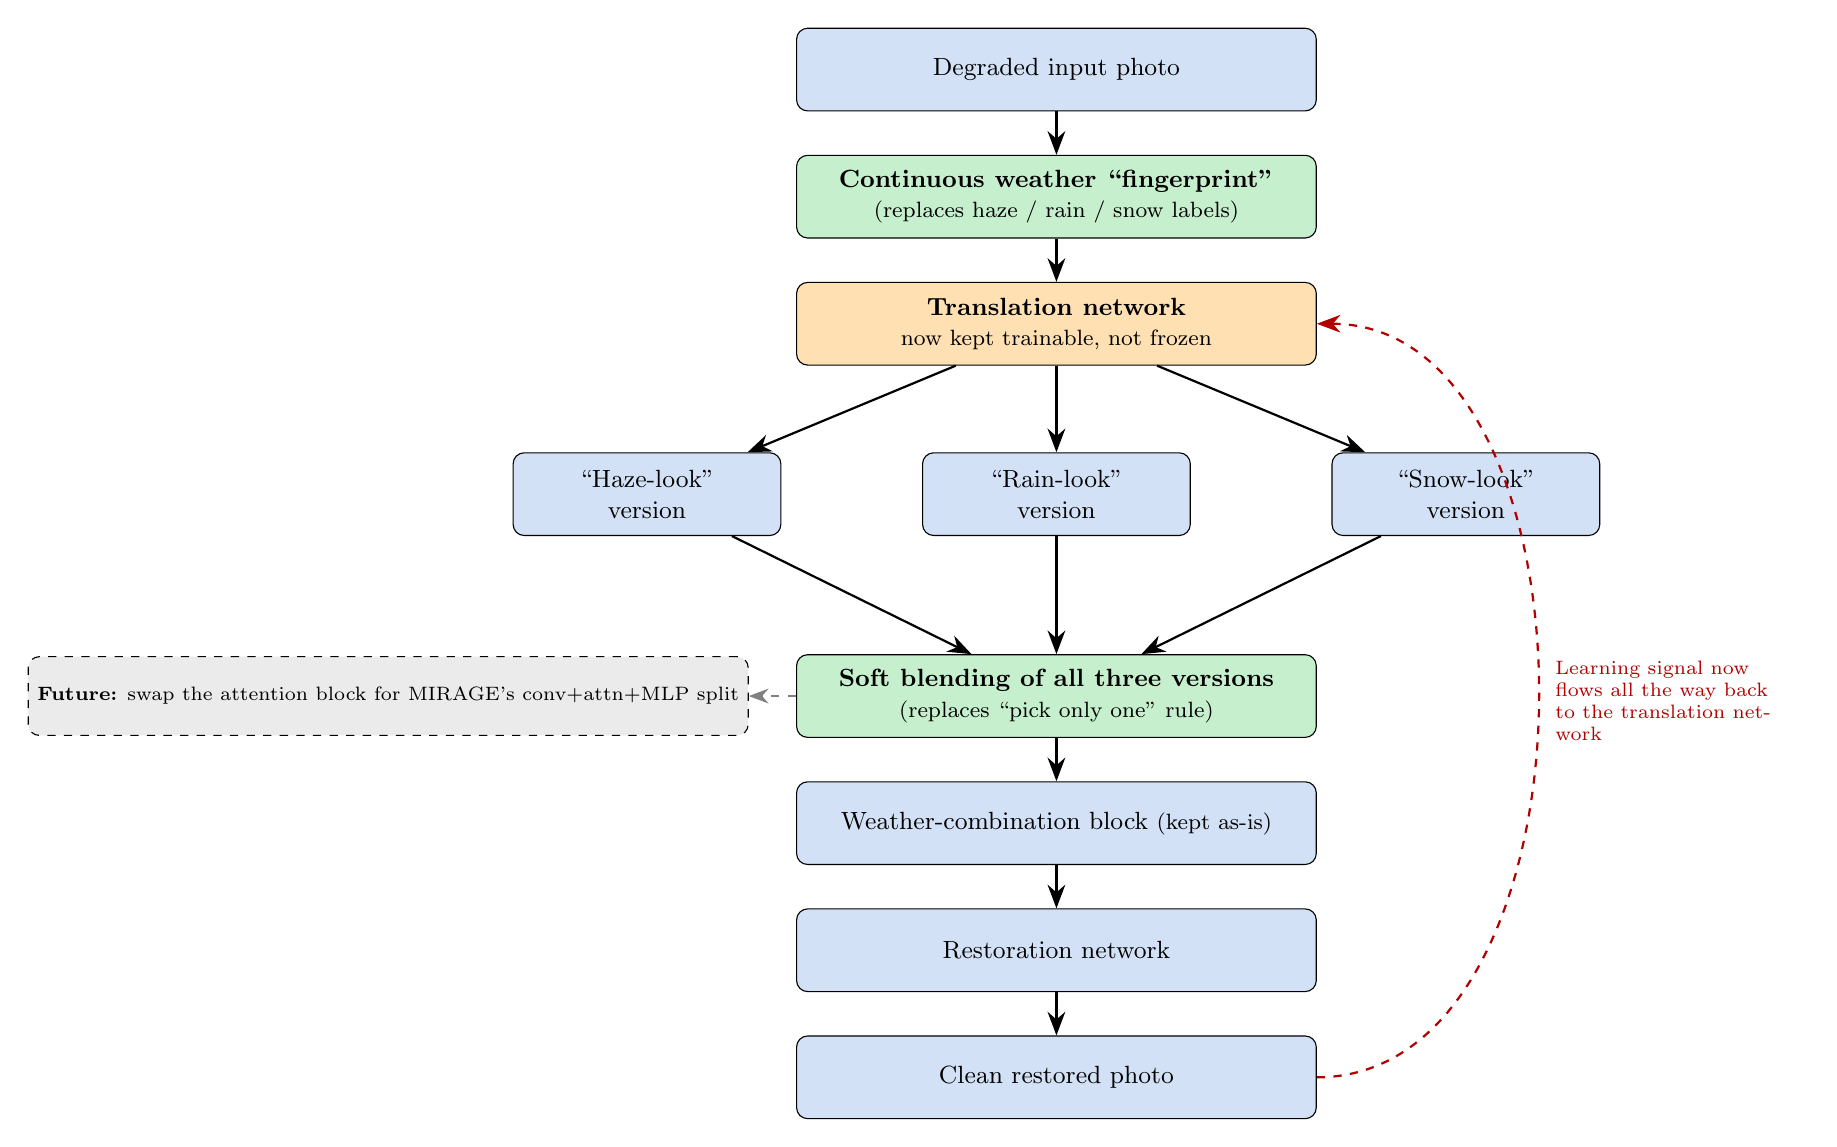
\begin{tikzpicture}[node distance=0.55cm]
\node[block, fill=kept] (input) {Degraded input photo};
\node[block, fill=newnode, below=of input] (embed)
  {\textbf{Continuous weather ``fingerprint''}\\ \footnotesize (replaces haze / rain / snow labels)};
\node[block, fill=changed, below=of embed] (translate)
  {\textbf{Translation network}\\ \footnotesize now kept trainable, not frozen};
\node[block, fill=kept, minimum width=3.4cm, below=1.1cm of translate, xshift=-5.2cm] (haze) {``Haze-look''\\version};
\node[block, fill=kept, minimum width=3.4cm, below=1.1cm of translate, xshift=0cm] (rain) {``Rain-look''\\version};
\node[block, fill=kept, minimum width=3.4cm, below=1.1cm of translate, xshift=5.2cm] (snow) {``Snow-look''\\version};
\node[block, fill=newnode, below=1.5cm of rain] (routing)
  {\textbf{Soft blending of all three versions}\\ \footnotesize (replaces ``pick only one'' rule)};
\node[block, fill=kept, below=of routing] (fusion) {Weather-combination block \footnotesize (kept as-is)};
\node[block, fill=kept, below=of fusion] (restore) {Restoration network};
\node[block, fill=kept, below=of restore] (output) {Clean restored photo};

\node[futureblock, left=0.6cm of routing] (ext1)
  {\textbf{Future:} swap the attention block for MIRAGE's conv+attn+MLP split};

\draw[arrowline] (input) -- (embed);
\draw[arrowline] (embed) -- (translate);
\draw[arrowline] (translate) -- (haze);
\draw[arrowline] (translate) -- (rain);
\draw[arrowline] (translate) -- (snow);
\draw[arrowline] (haze) -- (routing);
\draw[arrowline] (rain) -- (routing);
\draw[arrowline] (snow) -- (routing);
\draw[arrowline] (routing) -- (fusion);
\draw[arrowline] (fusion) -- (restore);
\draw[arrowline] (restore) -- (output);

\draw[dashedline] (output.east) to[out=0,in=0] node[right, xshift=1mm, font=\scriptsize, text width=3.1cm, align=left]
  {Learning signal now flows all the way back to the translation network} (translate.east);
\draw[futureline] (routing.west) -- (ext1.east);
\end{tikzpicture}
}
\end{frame}

\begin{frame}{How to Read the Flowchart}
\begin{columns}[T]
\begin{column}{0.32\textwidth}
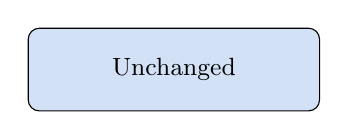
\begin{tikzpicture}
\node[block, fill=kept, minimum width=3.7cm] {Unchanged};
\end{tikzpicture}
\vspace{2mm}
Parts of DTMIR-Pro we are keeping exactly as they are --- they already work well.
\end{column}
\begin{column}{0.32\textwidth}
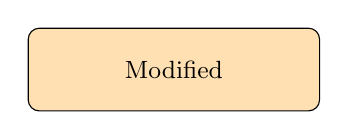
\begin{tikzpicture}
\node[block, fill=changed, minimum width=3.7cm] {Modified};
\end{tikzpicture}
\vspace{2mm}
An existing DTMIR-Pro part that we're changing how it behaves (not replacing it entirely).
\end{column}
\begin{column}{0.32\textwidth}
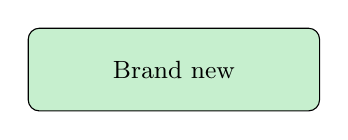
\begin{tikzpicture}
\node[block, fill=newnode, minimum width=3.7cm] {Brand new};
\end{tikzpicture}
\vspace{2mm}
A component that didn't exist in DTMIR-Pro at all --- newly added, inspired by another paper.
\end{column}
\end{columns}
\vspace{3mm}
\textcolor{red!70!black}{\bf Dashed red arrow:} information that now flows \emph{backward}
during training (a ``feedback loop'') --- this did not exist in the original pipeline.\\[2mm]
\small \textbf{Dashed gray box:} optional extension, added as a
\emph{future} node (MIRAGE backbone swap) --- not part of the current run.
\end{frame}

\begin{frame}{Change 1 --- A ``Fingerprint'' Instead of a Label}
\textbf{What it replaces:} DTMIR-Pro tags every image with a rigid label: haze,
rain, \emph{or} snow. Nothing in between.

\vspace{3mm}
\textbf{What we're doing instead:} Give every image a flexible, learned description
of its weather condition --- more like a fingerprint than a checkbox. This lets the
network say ``this photo is somewhat rainy and somewhat hazy'' instead of forcing a
single choice.

\vspace{3mm}
\textbf{Where the idea comes from:} The BDG paper (ICLR'26) uses a similar idea ---
instead of a fixed label for the type of damage in an image, it builds a rich,
learned description of the damage and feeds that into its model. We're borrowing
that same philosophy for weather type.

\vspace{3mm}
\textbf{Why it matters:} Real bad-weather photos are almost never purely one thing
--- a rainy evening often also looks hazy. A single label can't capture that; a
fingerprint can.
\end{frame}

\begin{frame}{Change 2 --- Letting the Translator Learn From the Outcome}
\textbf{What it replaces:} In DTMIR-Pro, the part of the network that creates the
haze/rain/snow versions of the image is trained \emph{once}, then locked. The later
restoration step can never tell it ``you got that a bit wrong, adjust.''

\vspace{3mm}
\textbf{What we're doing instead:} Keep that part unlocked during training, so the
quality of the final restored photo can send feedback backward and improve how the
translations are made in the first place.

\vspace{3mm}
\textbf{Where the idea comes from:} This is \emph{our own proposal}. The reading-list
papers gave us the general direction (they all re-use feedback across stages rather
than trusting one frozen pass blindly), but none of them makes this exact change, so
we are not attributing it to a specific paper.

\vspace{3mm}
\textbf{Why it matters:} A part of the system that never learns from its own
mistakes is wasted potential --- this closes that loop.
\end{frame}

\begin{frame}{Change 3 --- Blending Instead of Picking One}
\textbf{What it replaces:} DTMIR-Pro looks at the three translated versions
(haze/rain/snow look-alikes), measures which one looks least like the original photo,
and keeps \emph{only that one}. The other two are thrown away completely.

\vspace{3mm}
\textbf{What we're doing instead:} Keep all three, but assign each one a
learned ``how useful is this'' weight, and blend them together instead of
picking a winner. The soft blending layer itself is \emph{our own design}.

\vspace{3mm}
\textbf{Where the idea comes from:} MIRAGE (ICLR'26) does not do stream routing,
but it does propose a \emph{covariance (SPD) similarity} between feature streams.
That similarity idea is what we can borrow as the \emph{routing score} in a later
step; the blend layer around it is ours.

\vspace{3mm}
\textbf{Why it matters:} Throwing away two-thirds of your information on a rigid
rule is wasteful, and the rule itself has no way to improve during training.
\end{frame}

\begin{frame}{What We Looked At but Are \emph{Not} Using Right Now}
\begin{center}
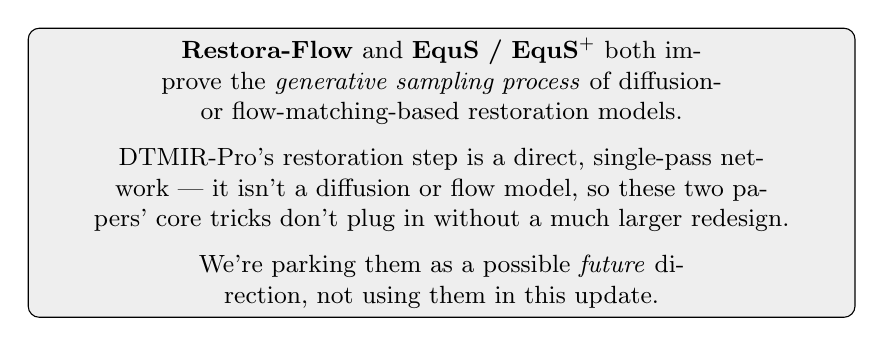
\begin{tikzpicture}
\node[block, fill=sidebox, minimum width=10.5cm, minimum height=2.6cm, text width=10cm]
{
\textbf{Restora-Flow} and \textbf{EquS / EquS$^+$} both improve the \emph{generative
sampling process} of diffusion- or flow-matching-based restoration models.\\[2mm]
DTMIR-Pro's restoration step is a direct, single-pass network --- it isn't a
diffusion or flow model, so these two papers' core tricks don't plug in without a
much larger redesign.\\[2mm]
We're parking them as a possible \emph{future} direction, not using them in this
update.
};
\end{tikzpicture}
\end{center}
\vspace{4mm}
This is intentional: it keeps the current update focused and realistic instead of
combining every paper into one giant redesign.
\end{frame}

\begin{frame}{What We Fixed in Code This Update}
\begin{itemize}
  \item \textbf{Stage-1 checkpoint now loads.} \texttt{train.py} no longer starts
  stage 2 from a fresh translator --- it loads \texttt{translator\_pretrained.pt}
  (with the weather embedding / projection), then freezes or fine-tunes as configured.
  \item \textbf{Parameter budget matched to the paper.} Baseline now sits at
  \textbf{3.93M params} (paper: 3.9M) by tuning \texttt{base\_channels=26},
  \texttt{num\_scales=3}.
  \item \textbf{Library SSIM} (torchmetrics) replaces the hand-written version.
  \item \textbf{Restoration net corrected to match the paper.} Re-reading the paper
  showed SBFR routes the \emph{last} translation-encoder layer (one feature map),
  upsampled into each decoder level next to three per-level MWF encoder branches
  (paper Eq.~8 and 11). Rewrote the restorer to match this instead of the earlier
  simplified single-branch decoder.
  \item \textbf{Cleaner soft-router input} via a small independent stem, replacing
  the old ``reuse the translator encoder'' shortcut.
  \item \textbf{Real training loop}: cosine-annealing LR, checkpointing, PSNR/SSIM
  validation, and CSV logging.
\end{itemize}
\end{frame}

\begin{frame}{First Visual Result: Smoke Training Curve}
\centering
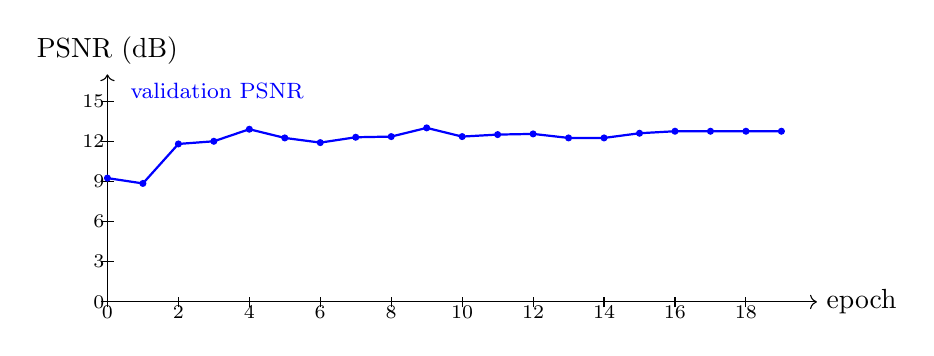
\begin{tikzpicture}[scale=0.85]
  \draw[->] (0,0) -- (0,3.4) node[above]{PSNR (dB)};
  \draw[->] (0,0) -- (10.6,0) node[right]{epoch};
  \foreach \y/\lab in {0/0, 0.6/3, 1.2/6, 1.8/9, 2.4/12, 3.0/15}
    \draw (-0.1,\y) -- (0.1,\y) node[left, font=\scriptsize]{\lab};
  \foreach \x in {0,2,4,6,8,10,12,14,16,18}
    \draw (\x*0.53,-0.08) -- (\x*0.53,0.08) node[below, font=\scriptsize]{\x};
  \draw[blue, thick] plot[mark=*, mark size=1pt] coordinates {
    (0.00,1.85) (0.53,1.77) (1.06,2.36) (1.59,2.40) (2.12,2.58)
    (2.65,2.45) (3.18,2.38) (3.71,2.46) (4.24,2.47) (4.77,2.60)
    (5.30,2.47) (5.83,2.50) (6.36,2.51) (6.89,2.45) (7.42,2.45)
    (7.95,2.52) (8.48,2.55) (9.01,2.55) (9.54,2.55) (10.07,2.55)
  };
  \node[anchor=west, blue] at (0.2,3.15) {\footnotesize validation PSNR};
\end{tikzpicture}
\vspace{2mm}

\small This is a \textbf{synthetic, CPU-only smoke run} (16 images, 64$\times$64, 20
epochs) --- the numbers are not comparable to the paper. It proves the full
\textbf{stage-1 $\rightarrow$ stage-2 pipeline learns end-to-end}: validation PSNR
climbs $\approx 8.9 \to 12.7$ dB and SSIM $0.23 \to 0.48$.
\end{frame}

\begin{frame}{The Ablation Ladder We Can Now Run}
\footnotesize
\begin{tabular}{l l l l c c}
\toprule
\textbf{Row} & \textbf{Weather code} & \textbf{Translator} & \textbf{Routing} & \textbf{PSNR} & \textbf{SSIM} \\
\midrule
B0 (baseline) & one-hot & frozen & hard & --- & --- \\
B1 & one-hot & trainable & hard & --- & --- \\
B2 & continuous & frozen & hard & --- & --- \\
B3 & one-hot & frozen & soft & --- & --- \\
B4 (full) & continuous & trainable & soft & --- & --- \\
\bottomrule
\end{tabular}
\vspace{3mm}

\begin{itemize}
  \item The runner (\texttt{run\_ablation.py}) is written and \textbf{verified} end-to-end
  on synthetic data --- it pretrains the translator once per weather-code mode, runs all
  five rows, and writes one comparable table.
  \item Each row answers ``which of the three changes was actually worth it'', including
  the possibility that soft routing helps little.
  \item Reference from the DTMIR-Pro paper (SOTS): \textbf{PSNR 36.92 / SSIM 0.981}.
  \item Real numbers need a GPU + the SOTS/ORD/CSD datasets (next slide).
\end{itemize}
\end{frame}

\begin{frame}{What We Need Next}
\begin{itemize}
  \item \textbf{GPU access.} A Colab notebook (\texttt{colab\_train.ipynb}) is ready;
  the paper used a GTX 1080 8GB, so any Colab T4 is enough.
  \item \textbf{Datasets.} SOTS (haze), Outdoor-Rain ORD, Comprehensive Snow CSD ---
  ideally a small subset first to get a first curve, then the full sets.
  \item \textbf{One decision for the advisor:} is a reproduction \emph{slightly under}
  the paper's numbers acceptable as our baseline row, or do we compare only against our
  own re-trained baselines?
\end{itemize}

\vspace{2mm}
\textbf{Known gaps we are flagging honestly:}
\begin{itemize}
  \item The contrastive loss uses a \texttt{pos/neg} ratio that can blow up when the
  translated streams are too similar --- we will re-check it against the paper.
  \item The continuous weather embedding has no auxiliary supervision yet.
  \item Real-world (RTTS/RID/Snow-Realistic) NIQE/Entropy/BRISQUE evaluation is later.
\end{itemize}
\end{frame}

\begin{frame}{Summary Table}
\footnotesize
\renewcommand{\arraystretch}{1.3}
\begin{tabular}{p{2.05cm}p{2.55cm}p{1.65cm}p{2.55cm}}
\toprule
\textbf{Change} & \textbf{Replaces} & \textbf{Inspired by} & \textbf{Benefit} \\
\midrule
Continuous weather fingerprint & Fixed haze/rain/snow label & BDG (ICLR'26) &
Handles mixed real-world weather \\
\addlinespace
Unfrozen translator & Frozen, one-time-trained translator & Our own proposal &
Translator improves alongside restoration \\
\addlinespace
Soft blending of streams & Hard ``pick one, discard two'' rule & Own design (+ MIRAGE SPD idea) &
No information thrown away; trainable \\
\bottomrule
\end{tabular}
\vspace{4mm}

\small Considered but deferred: Restora-Flow, EquS/EquS$^+$ (both assume a
diffusion/flow-based restorer, which DTMIR-Pro is not).
\end{frame}

\begin{frame}
\centering
\Large Thank you --- Questions / Discussion
\end{frame}

\end{document}
